\documentclass[compress]{beamer}
\setbeamercovered{transparent}
\usepackage[utf8]{inputenc}


\usepackage{multirow,rotating}
\usepackage{color}
\usepackage{hyperref}
\usepackage{tikz-cd}
\usepackage{array}
\usepackage{siunitx}
\usepackage{mathtools,nccmath}%
\usepackage{etoolbox, xparse}
\usepackage{adjustbox}
\usetheme{CambridgeUS}
\usecolortheme{dolphin}
%%%%%%%%%%%%%%%%%%%%%%%%%%%%%%%%%%%%%%%%%%%%%%%%%%%%%%%%%%%%%%%%%%%%%%%%%%%%%%
% \embedvideo{<poster or text>}{<video file (MP4+H264)>}
% \embedvideo*{...}{...}                     % auto-play
%%%%%%%%%%%%%%%%%%%%%%%%%%%%%%%%%%%%%%%%%%%%%%%%%%%%%%%%%%%%%%%%%%%%%%%%%%%%%%

\usepackage[bigfiles]{pdfbase}
\ExplSyntaxOn
\NewDocumentCommand\embedvideo{smm}{
  \group_begin:
  \leavevmode
  \tl_if_exist:cTF{file_\file_mdfive_hash:n{#3}}{
    \tl_set_eq:Nc\video{file_\file_mdfive_hash:n{#3}}
  }{
    \IfFileExists{#3}{}{\GenericError{}{File~`#3'~not~found}{}{}}
    \pbs_pdfobj:nnn{}{fstream}{{}{#3}}
    \pbs_pdfobj:nnn{}{dict}{
      /Type/Filespec/F~(#3)/UF~(#3)
      /EF~<</F~\pbs_pdflastobj:>>
    }
    \tl_set:Nx\video{\pbs_pdflastobj:}
    \tl_gset_eq:cN{file_\file_mdfive_hash:n{#3}}\video
  }
  %
%   \pbs_pdfobj:nnn{}{dict}{
%     /Type/RichMediaInstance/Subtype/Video
%     /Asset~\video
%     /Params~<</FlashVars (
%       source=#3&
%       skin=SkinOverAllNoFullNoCaption.swf&
%       skinAutoHide=true&
%       skinBackgroundColor=0x5F5F5F&
%       skinBackgroundAlpha=0&
%       loop=true
%     )>>
%   }
  \pbs_pdfobj:nnn{}{dict}{
    /Type/RichMediaInstance/Subtype/Video
    /Asset~\video
    /Params~<</FlashVars (
      source=#3&
      skin=SkinOverAllNoFullNoCaption.swf&
      skinAutoHide=true&
      skinBackgroundColor=0x5F5F5F&
      skinBackgroundAlpha=0.75&
      loop=true
    )>>
  }
  %
  \pbs_pdfobj:nnn{}{dict}{
    /Type/RichMediaConfiguration/Subtype/Video
    /Instances~[\pbs_pdflastobj:]
  }
  %
  \pbs_pdfobj:nnn{}{dict}{
    /Type/RichMediaContent
    /Assets~<<
      /Names~[(#3)~\video]
    >>
    /Configurations~[\pbs_pdflastobj:]
  }
  \tl_set:Nx\rmcontent{\pbs_pdflastobj:}
  %
  \pbs_pdfobj:nnn{}{dict}{
    /Activation~<<
      /Condition/\IfBooleanTF{#1}{PV}{XA}
      /Presentation~<</Style/Embedded>>
    >>
    /Deactivation~<</Condition/PI>>
  }
  %
  \hbox_set:Nn\l_tmpa_box{#2}
  \tl_set:Nx\l_box_wd_tl{\dim_use:N\box_wd:N\l_tmpa_box}
  \tl_set:Nx\l_box_ht_tl{\dim_use:N\box_ht:N\l_tmpa_box}
  \tl_set:Nx\l_box_dp_tl{\dim_use:N\box_dp:N\l_tmpa_box}
  \pbs_pdfxform:nnnnn{1}{1}{}{}{\l_tmpa_box}
  %
  \pbs_pdfannot:nnnn{\l_box_wd_tl}{\l_box_ht_tl}{\l_box_dp_tl}{
    /Subtype/RichMedia
    /BS~<</W~0/S/S>>
    /Contents~(embedded~video~file:#3)
    /NM~(rma:#3)
    /AP~<</N~\pbs_pdflastxform:>>
    /RichMediaSettings~\pbs_pdflastobj:
    /RichMediaContent~\rmcontent
  }
  
  \phantom{#2}
  \group_end:
}
\ExplSyntaxOff
%%%%%%%%%%%%%%%%%%%%%%%%%%%%%%%%%%%%%%%%%%%%%%%%%%%%%%%%%%%%%%%%%%%%%%%%%%%%%%
\usepackage{graphics}
\usepackage{media9}
\usepackage{graphicx}

% set colors
\definecolor{myNewColorA}{RGB}{158, 27,50}   % wine red
\definecolor{myNewColorB}{RGB}{225, 225,225} % white
\definecolor{myNewColorC}{RGB}{242, 242,242} % {130,138,143}
\setbeamercolor*{palette primary}{bg=myNewColorA}
\setbeamercolor*{palette secondary}{bg=myNewColorA, fg = white}
\setbeamercolor*{palette tertiary}{bg=myNewColorA, fg = white}
\setbeamercolor*{titlelike}{fg=myNewColorA}
\setbeamercolor*{title}{bg=myNewColorA, fg = white}
\setbeamercolor*{item}{fg=myNewColorA}
\setbeamercolor*{caption name}{fg=myNewColorA}
\setbeamercolor*{block title}{fg=white, bg = myNewColorA}
\setbeamercolor*{block body}{bg = myNewColorC}
\usefonttheme{professionalfonts}
\setbeamercolor*{subsection in head/foot}{bg=myNewColorB,fg=black}
\setbeamercolor{page number in head/foot}{fg=myNewColorB}


\setbeamertemplate{headline}{%
  \begin{beamercolorbox}[colsep=1.5pt]{upper separation line head}
  \end{beamercolorbox}
  \begin{beamercolorbox}{section in head/foot}
    \vskip-0.2pt\insertnavigation{\paperwidth}\vskip2pt
  \end{beamercolorbox}%
  \begin{beamercolorbox}[colsep=1.5pt]{lower separation line head}
  \end{beamercolorbox}
}
\makeatother

\setbeamertemplate{bibliography item}[text]

\setbeamertemplate{frametitle}{%
    \nointerlineskip%
    \begin{beamercolorbox}[wd=\paperwidth,ht=25pt,dp = 1pt]{frametitle}
        \hspace*{10pt}\insertframetitle\vskip5pt
    \end{beamercolorbox}%
}

% Author, title, note
\setbeamercolor{bibliography entry author}{fg=myNewColorA}
\setbeamercolor{bibliography entry title}{fg=myNewColorA}
\setbeamercolor{bibliography entry note}{fg=myNewColorA}
\usepackage{hyperref}

\titlegraphic{%

\includegraphics[width=2cm]{UvA.png}
}
% set font size
\setbeamerfont{title}{size=\Large}
\setbeamerfont{subtitle}{size=\large}
\setbeamerfont{author}{size=\large}
\setbeamerfont{date}{size=\small}
\setbeamerfont{institute}{size=\large}
\setbeamerfont{block title}{size=\normalsize}
\setbeamerfont{block body}{size=\footnotesize}
\title[Agent-based Modeling]{Agent-based Modeling}%title
\subtitle{}%%subtitle
\author[CCI]{Xin Zhou}
\institute[Informatics Institute]{University of Amsterdam}
\author[x.zhou@uva.nl]{Xin Zhou}%%authors
\institute[Informatics Institute]{University of Amsterdam}

\date[\textcolor{white}{Behavior Summer School, 2022}]
{Behavior Summer School on Agent-based Modelling for Social Science\\
29 Aug- 09 Sep, 2022}

%------------------------------------------------------------
%beginning of each section and highlights the current section:
%\AtBeginSection[]
%{
%  \begin{frame}
%    \frametitle{Contents}
%    \tableofcontents[currentsection]
%  \end{frame}
%}
\AtBeginSection[]{
  \begin{frame}
  \vfill
  \centering
  \begin{beamercolorbox}[sep=8pt,center,shadow=true,rounded=true]{title}
    \usebeamerfont{title}\insertsectionhead\par%
  \end{beamercolorbox}
  \vfill
  \end{frame}
}

% ---- Citations ------------
\usepackage{filecontents}
\begin{filecontents}{bibexample.bib}
@book{gilbert2005simulation,
  title={Simulation for the social scientist},
  author={Gilbert, Nigel and Troitzsch, Klaus},
  year={2005},
  publisher={McGraw-Hill Education (UK)}
}

@article{schelling1971dynamic,
  title={Dynamic models of segregation},
  author={Schelling, Thomas C},
  journal={Journal of mathematical sociology},
  volume={1},
  number={2},
  pages={143--186},
  year={1971},
  publisher={Taylor \& Francis}
}

@article{manzo2018complex,
  title={Complex contagions and the diffusion of innovations: Evidence from a small-N study},
  author={Manzo, Gianluca and Gabbriellini, Simone and Roux, Valentine and M’mbogori, Freda Nkirote},
  journal={Journal of Archaeological Method and Theory},
  volume={25},
  number={4},
  pages={1109--1154},
  year={2018},
  publisher={Springer}
}

@article{bravo2012trust,
  title={Trust and partner selection in social networks: An experimentally grounded model},
  author={Bravo, Giangiacomo and Squazzoni, Flaminio and Boero, Riccardo},
  journal={Social Networks},
  volume={34},
  number={4},
  pages={481--492},
  year={2012},
  publisher={Elsevier}
}

@article{zhou2022costly,
  title={Costly incentives design from an institutional perspective: cooperation, sustainability and affluence},
  author={Zhou, Xin and Belloum, Adam and Lees, Michael H and van Engers, Tom and de Laat, Cees},
  journal={Proceedings of the Royal Society A},
  volume={478},
  number={2265},
  pages={20220393},
  year={2022},
  publisher={The Royal Society}
}

\end{filecontents}

% ===================================================================
\usepackage[style=ieee,citetracker=true, backend=biber]{biblatex}
\addbibresource{bibexample.bib}


% ------Contents below------
\begin{document}

% The next statement creates the title page.
% \frame[plain]{\titlepage}
\begingroup
    \setbeamertemplate{headline}{}
    \begin{frame}
        \titlepage
    \end{frame}
\endgroup

%% If the content is not that much, can delete the table of content page
% \begin{frame}
% \frametitle{Outline}
% \tableofcontents
% \end{frame}

%------------------------------------------------------------
\section{Introduction}
\setbeamertemplate{background}
{
    
\includegraphics[width=\paperwidth,height=\paperheight]{UvA-bg.png}
}

\subsection{Definition}
\begin{frame}{What and why}
    \begin{itemize}
        \item<1-> What is ABM
            \begin{center}
                \begin{minipage}{10.3cm}
                \begin{block}{Agent-based models}
                    ABMs represent individuals, their \textbf{behaviors} and their \textbf{interactions}.
                \end{block}
                \end{minipage}
            \end{center}
        \item[] % add a space line
        \item<2-> Why we need ABM
            \begin{itemize}
                \item Heterogeneous individuals
                \item Sophisticated interactions
                \item Dynamic environment
            \end{itemize}
        \item<3> Social science simulation approaches\cite{gilbert2005simulation}
    \end{itemize}
\end{frame}

\begin{frame}{Development}
        \begin{figure}
            \centering
            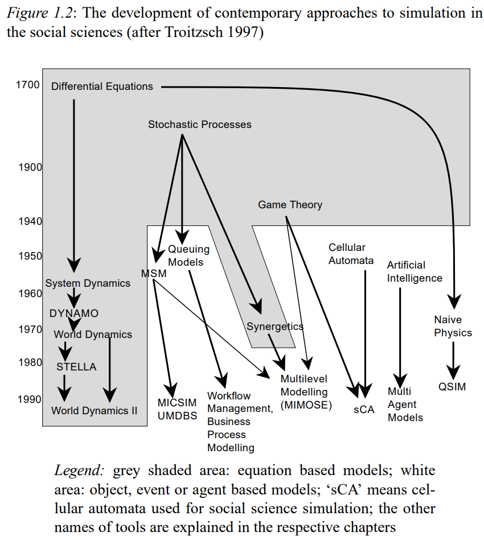
\includegraphics[scale=0.5]{SocialScienceSimDev.png}
            \label{fig:my_label}
        \end{figure}
\end{frame}

\subsection{Applications}
\begin{frame}{Applications}
    \begin{itemize}
        \item<1-> Computational Social Science
        \item<2-> Public health / Politics
        \item<3-> Economics / Marketing
        \item<4-> Management / Operation Research
        \item<5-> Microbiology
        \item<5-> ...
    \end{itemize}
\end{frame}

\section{Research Paradigm}
\subsection{Explanation examples}
\begin{frame}{Explanation: \href{https://github.com/CinkerZX/BasicNetLogoSimModels}{Shelling model\cite{schelling1971dynamic}}}

    \begin{columns}[c]
    % create the column with the first image, that occupies
    % half of the slide
        \begin{column}{.4\textwidth}
            \centering
            \embedvideo{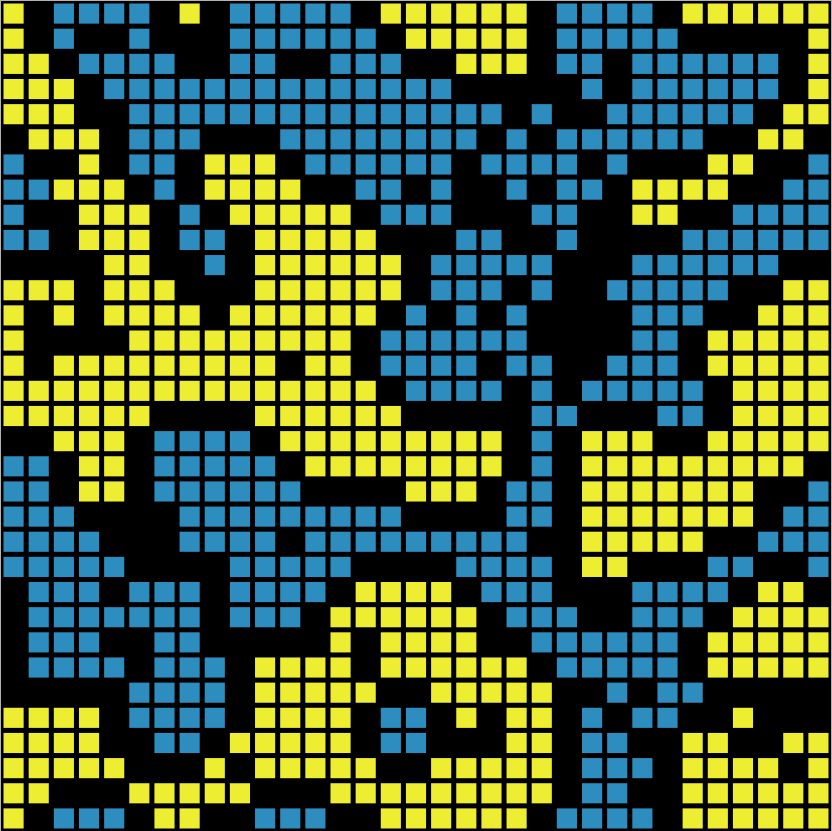
\includegraphics[width=\textwidth]{ShellingModel.png}}{ShellingModel.mp4}
        \end{column}
    % create the column with the second image, that also
    % occupies half of the slide
        \begin{column}{.5\textwidth}
            \raggedright
            \begin{minipage}{5.8cm}
                \begin{block}{Research question}
                    What is the mechanism of forming the highly segregated society?
                \end{block}
                \begin{block}{Modeling}
                    \textbf{Micro-motives}:\\
                    \begin{itemize}
                        \item Agents desire a fraction $ p_a $ of their neighbors to be of the same group
                        \item Check better empty spaces ($ p > p_{a} $) to move to, until everyone is satisfied
                    \end{itemize}
                    \textbf{Macro-behavior}: Segregation
                \end{block}
            \end{minipage}
        \end{column}
    \end{columns}
\end{frame}

\begin{frame}{Explanation: \href{https://github.com/CinkerZX/circles-and-squares}{Innovation Diffusion model\cite{manzo2018complex}}}
    \begin{columns}[c]
    % create the column with the first image, that occupies
    % half of the slide
        \begin{column}{.5\textwidth}
            \centering
            \embedvideo{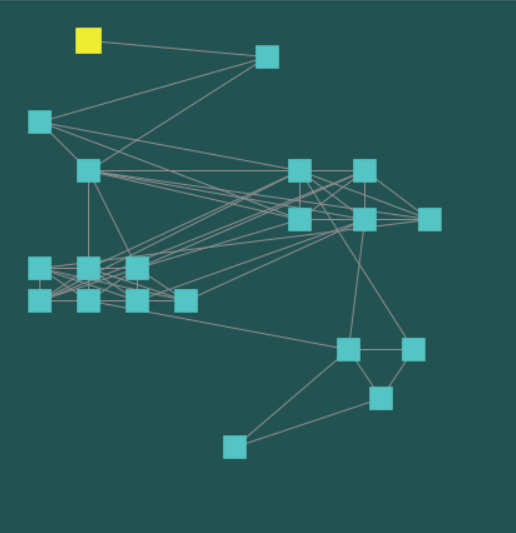
\includegraphics[width=0.6\textwidth]{InnovationDiffusionModel-1.png}}{InnovationDiffusionModel-1.mp4} \\
            \embedvideo{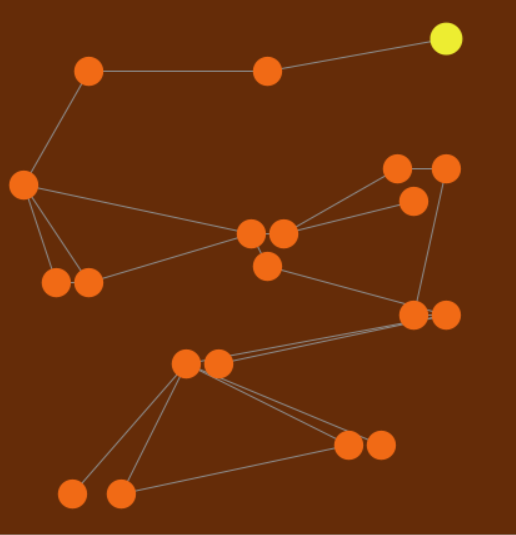
\includegraphics[width=0.6\textwidth]{InnovationDiffusionModel-2.png}}{InnovationDiffusionModel-2.mp4}
        \end{column}
    % create the column with the second image, that also
    % occupies half of the slide
        \begin{column}{.5\textwidth}
            \raggedright
            \begin{minipage}{5.8cm}
                \begin{block}{Research question}
                    What creates the difference in innovation diffusion in different ethnic group?
                \end{block}
                \begin{block}{Modeling}
                    \textbf{Diffusion mechanism}:\\
                    \begin{itemize}
                        \item Randomly (base line)
                        \item Geodesic distance (Contact network)
                        \item Kinship distance
                        \item \#Links between common neighbors
                        \item $\frac{\text{\footnotesize \#adopter in neighbor}}{\text{\footnotesize \#neighbors}}$
                    \end{itemize}
                    \textbf{Calibration}: Which mechanism fits the real data best
                \end{block}
            \end{minipage}
        \end{column}
    \end{columns}
\end{frame}

\begin{frame}{\href{https://www.sciencedirect.com/science/article/pii/S0378873312000202}{Prediction: Influence of selection on cooperation\cite{bravo2012trust}}}

    \begin{columns}[c]
    % create the column with the first image, that occupies
    % half of the slide
        \begin{column}{.5\textwidth}
            \centering
            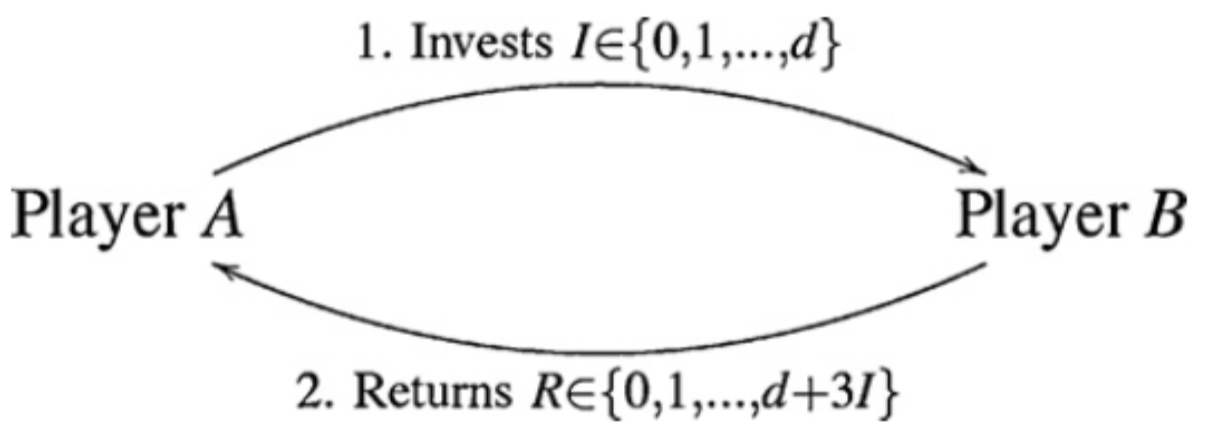
\includegraphics[width=0.8\textwidth]{InvestmentGame.png}\\[0.5cm]
            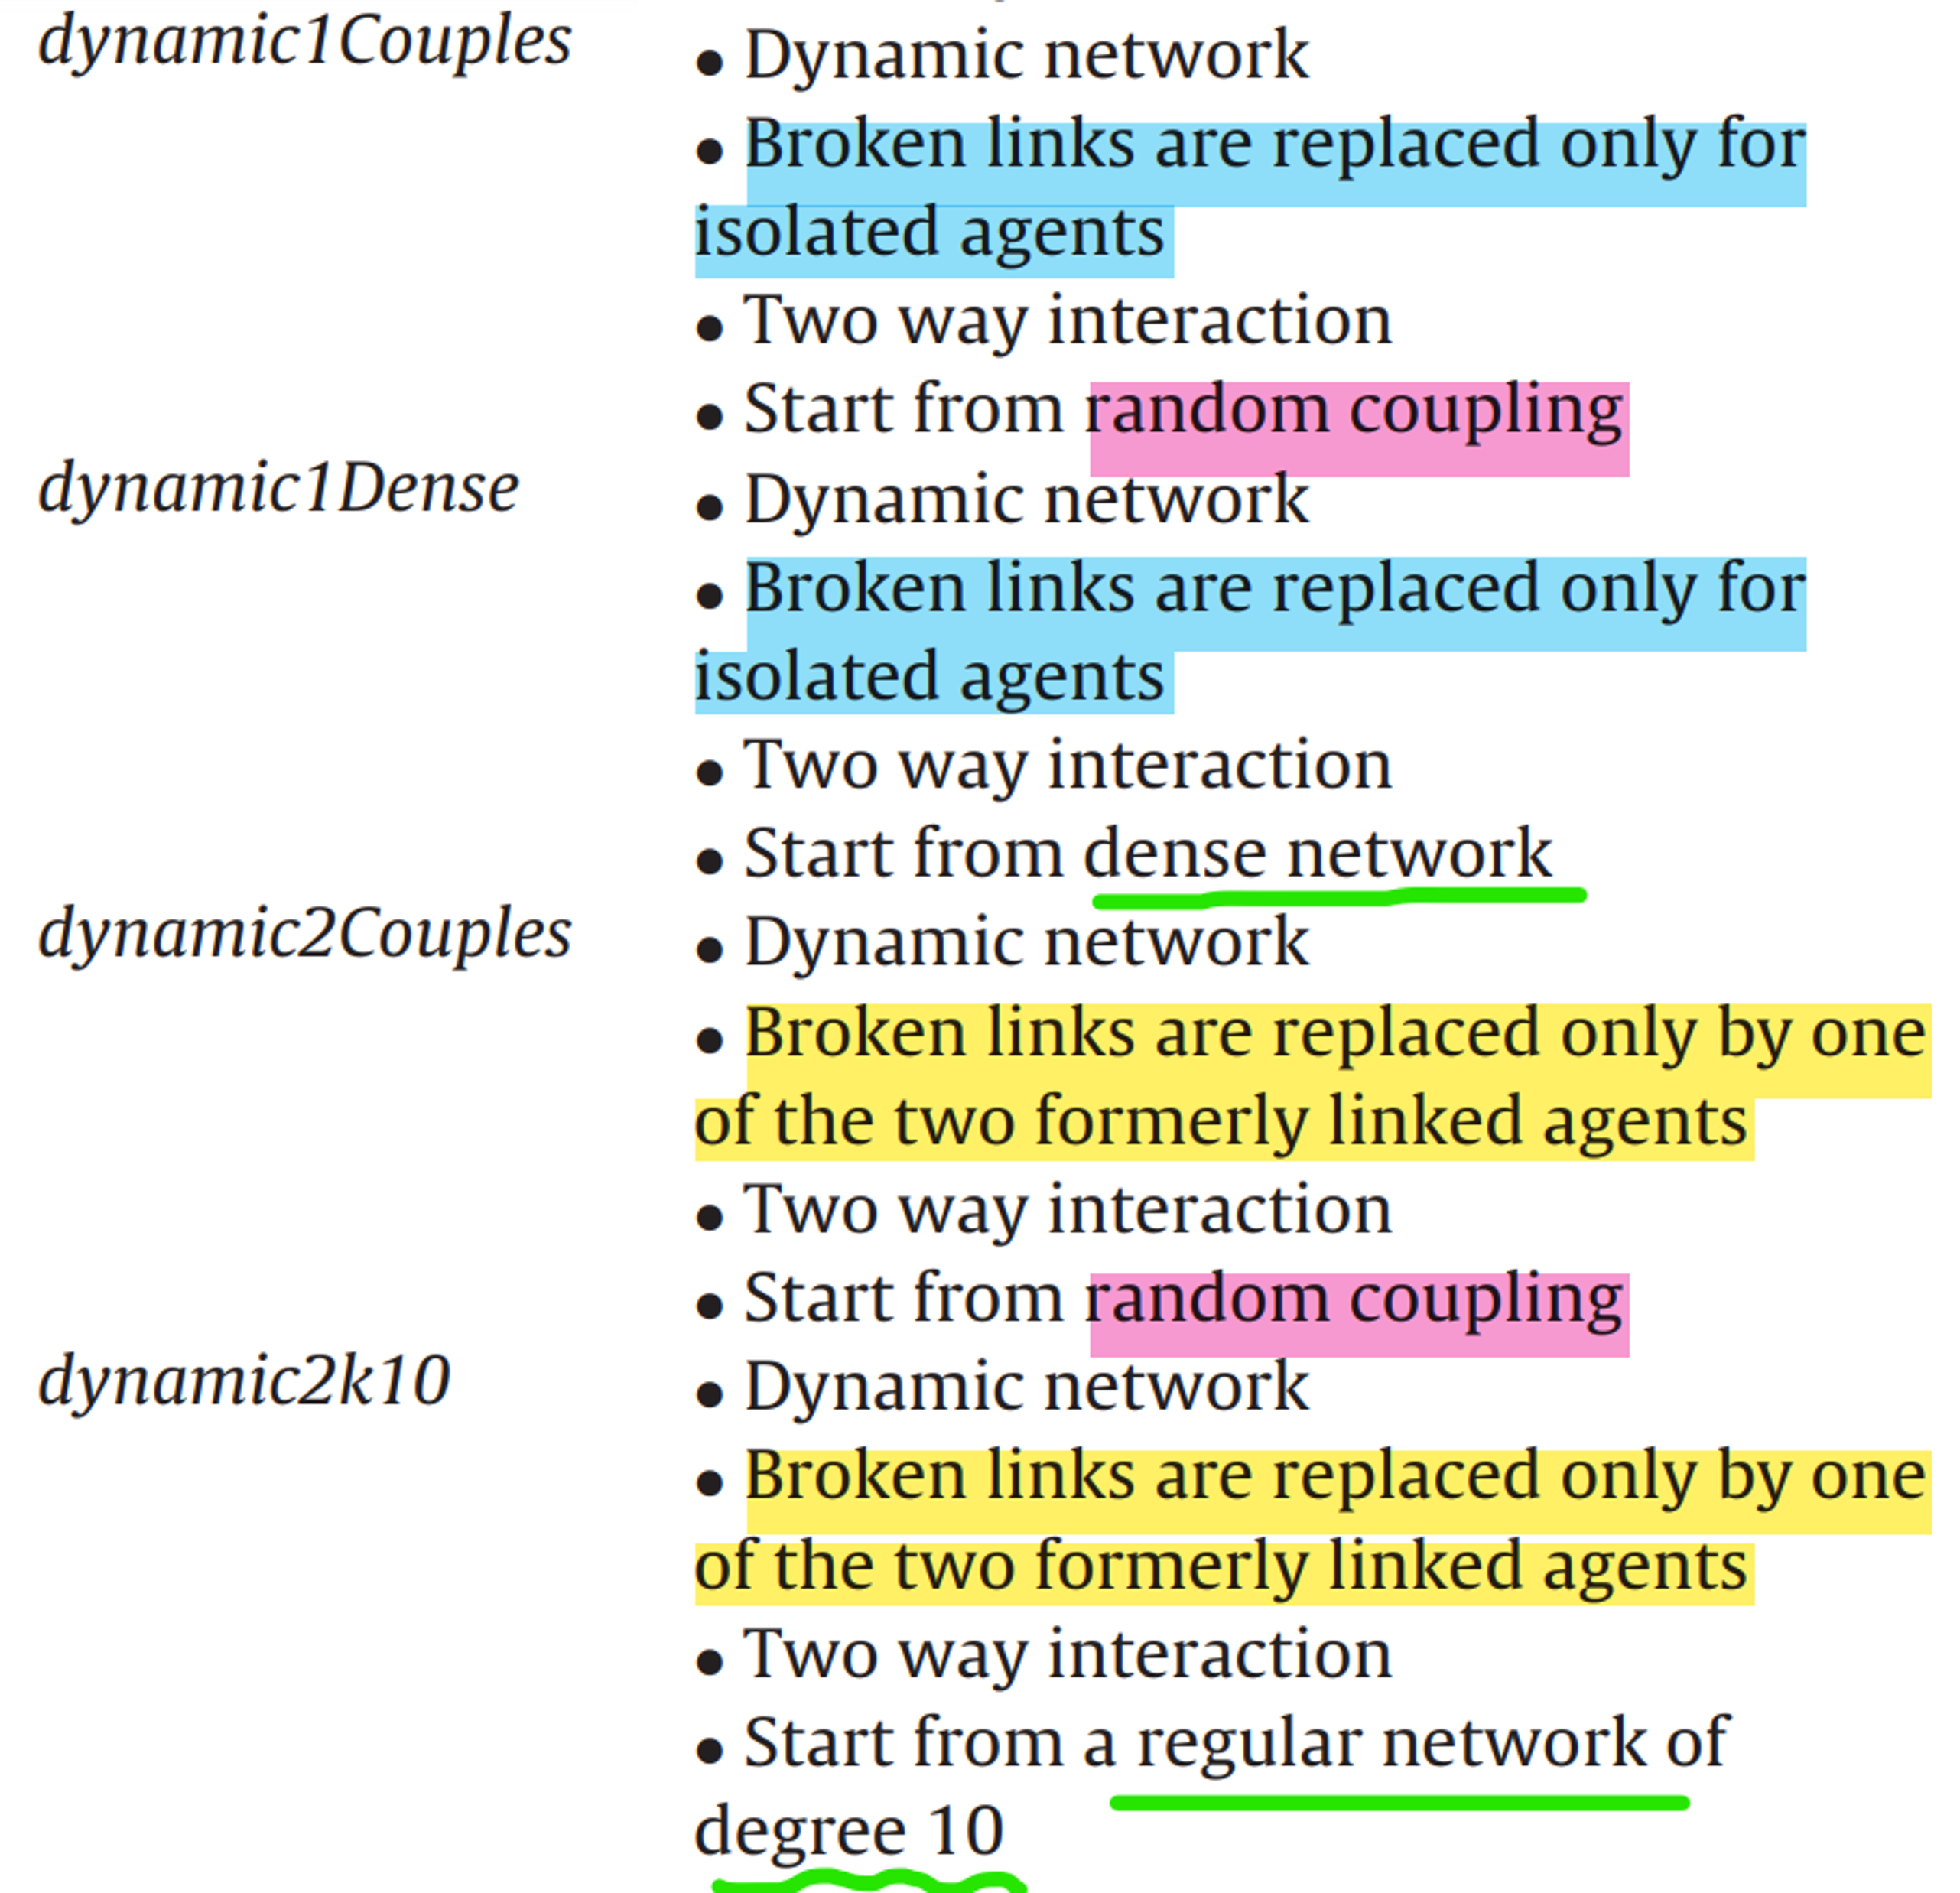
\includegraphics[width=0.8\textwidth]{ABMExp.png}
        \end{column}
    % create the column with the second image, that also
    % occupies half of the slide
        \begin{column}{.5\textwidth}
            \raggedright
            \begin{minipage}{5.8cm}
                \begin{block}{Research question}
                    What is the mechanism of forming the highly segregated society?
                \end{block}
                \begin{block}{Research Method}
                    \textbf{Lab experiment}:\\
                    \begin{itemize}
                        \item Play repeated investment game
                        \item Record behavior, calibrate trusting preference $ \alpha_{i} $, trustworthiness $ \gamma_{i} $
                    \end{itemize}
                    \textbf{ABM}:
                    \begin{itemize}
                        \item Design different interaction mechanism
                        \item Predict and evaluate the influence of selection
                    \end{itemize}
                \end{block}
            \end{minipage}
        \end{column}
    \end{columns}
\end{frame}
%*********************************
\subsection{Prediction examples}
\begin{frame}{\href{https://royalsocietypublishing.org/doi/full/10.1098/rspa.2022.0393}{Prediction: Proper Incentive Design~\cite{zhou2022costly}}}
    \begin{columns}[c]
    % create the column with the first image, that occupies
    % half of the slide
        \begin{column}{.5\textwidth}
            \centering
            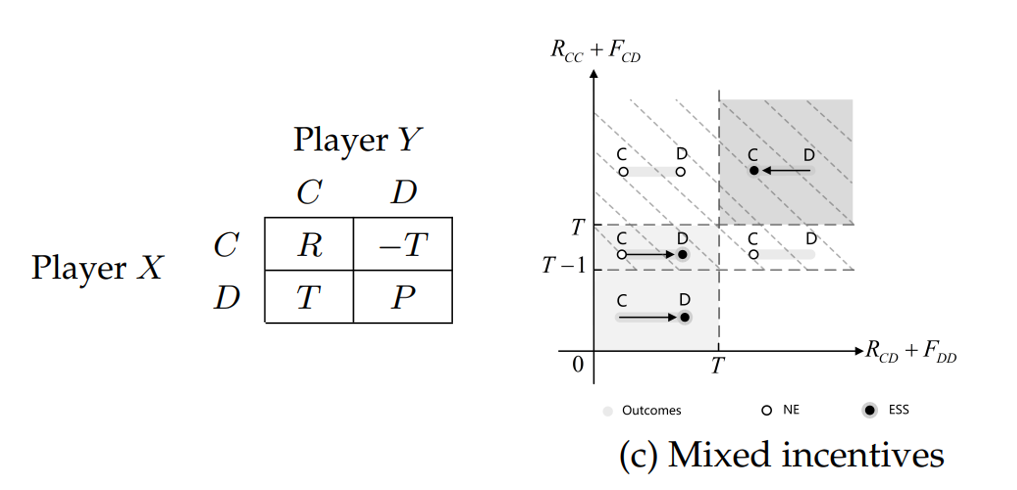
\includegraphics[width=\textwidth]{ProperIncentAnaModel.png}\\[0.5cm]
            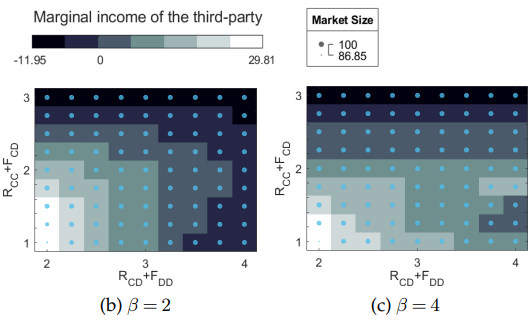
\includegraphics[width=0.9\textwidth]{ProperIncentExpResult.png}\\[0.5cm]
        \end{column}
    % create the column with the second image, that also
    % occupies half of the slide
        \begin{column}{.5\textwidth}
            \raggedright
            \begin{minipage}{5.8cm}
                \begin{block}{Research question}
                    Predicting the influence of incentives
                \end{block}
                \begin{block}{Research Method}
                    \textbf{Analytical solution}:\\
                    \begin{itemize}
                        \item Evolutionary Game Theory
                        \item Assumptions: rational agents; infinite population
                    \end{itemize}
                    \textbf{ABM}:
                    \begin{itemize}
                        \item Relax assumptions
                        \item Introduce income and cost for incentives executor
                        \item Elimination mechanism
                    \end{itemize}
                \end{block}
            \end{minipage}
        \end{column}
    \end{columns}
\end{frame}

\subsection{Summary}
\begin{frame}{Paradigm}
    \begin{itemize}
        \item<1-> Explanation
            \begin{itemize}
                \item \underline{Design model} (Theories, observations ...)
                \item Calibration by real dataset
                \\ \textcolor{gray}{Estimate the value of variables}
                \item Compare generated data with real data
                \\ \textcolor{gray}{To what extent your model can \textbf{explain} the real world}
                \item Robustness analysis
            \end{itemize}
        \item<2-> Prediction
            \begin{itemize}
                \item \underline{Design model} (Combine with other methods)
                \item \textbf{Predict} by the generated data
                \item \textcolor{myNewColorA}{Calibration?}
                \item \textcolor{myNewColorA}{Compare?}
            \end{itemize}
    \end{itemize}
\end{frame}

\section{Principles of model design}
\begin{frame}{K.I.S.S or K.I.D}
    \begin{itemize}
        \item<1-> \textcolor{myNewColorA}{\textbf{K}}eep \textcolor{myNewColorA}{\textbf{I}}t \textcolor{myNewColorA}{\textbf{S}}imple and \textcolor{myNewColorA}{\textbf{S}}tupid\\
        Ockham's Razor principle
        \item<2-> \textcolor{myNewColorA}{\textbf{K}}eep \textcolor{myNewColorA}{\textbf{I}}t \textcolor{myNewColorA}{\textbf{D}}escriptive\\
        The advantage of ABM
    \end{itemize}
\end{frame}

\begin{frame}{K.I.S.S or K.I.D}
    \begin{itemize}
        \item \textcolor{myNewColorA}{\textbf{K}}eep \textcolor{myNewColorA}{\textbf{I}}t \textcolor{myNewColorA}{\textbf{S}}imple and \textcolor{myNewColorA}{\textbf{S}}tupid\\
        Ockham's Razor principle
        \item \textcolor{myNewColorA}{\textbf{K}}eep \textcolor{myNewColorA}{\textbf{I}}t \textcolor{myNewColorA}{\textbf{D}}escriptive\\
        Advantage of ABM
    \end{itemize}
    \begin{center}
        \begin{minipage}{10cm}
            \begin{block}{No standard answer}
                Depends on the research question
            \end{block}
        \end{minipage}
    \end{center}
    
\end{frame}

\begin{frame}
	\printbibliography
\end{frame}

\begin{frame}
    \titlepage
\end{frame}

\end{document}



